\documentclass[11pt,english,compress]{beamer}
\usepackage[utf8]{inputenc}
\usepackage{smartdiagram}
\usepackage{verbatim}
\usepackage{eurosym}
\usepackage{stmaryrd}
\usepackage{subfig}

\useoutertheme{smoothbars}
\useinnertheme[shadow=true]{rounded}
\usecolortheme{orchid}
\usecolortheme{whale}
\title{EzBench, a tool to help you benchmark and bisect the Graphics Stack's performance}
\subtitle{}
\author{Martin Peres}
\institute{Intel Open Source Technology Center Finland}

\AtBeginSection[]{
  \begin{frame}{Summary}
  \small \tableofcontents[currentsection, hideothersubsections]
  \end{frame} 
}

\begin{document}

\setbeamertemplate{navigation symbols}{}

\begin{frame}
	\titlepage
\end{frame}

\section{Introduction}
\subsection*{Introduction}
\begin{frame}
	\frametitle{Introduction}

	\begin{block}{Current situation}
		\begin{itemize}
			\item Complex games/benchmarks are available and used on Linux;
			\item Drivers are getting more complex as performance improves;
			\item Users now rely on Open Source drivers for games/apps...
		\end{itemize}
	\end{block}
	
	\pause
	
	\begin{block}{Risks when merging new code}
		\begin{itemize}
			\item Break previous functionalities / rendering;
			\item Break the performance of a game inadvertly;
			\item Improve the performance of one app but slow down others.
		\end{itemize}
	\end{block}
	
	\pause
	
	\begin{block}{}
		$\Rightarrow$ Need to test and benchmark all the platforms and games of interest.
	\end{block}
\end{frame}

\section{Graphics Continuous Integration}
\subsection*{Objectives}
\begin{frame}
	\frametitle{CI: Objectives and chalenges}
	
	\begin{block}{Objectives}
		\begin{itemize}
			\item Catch changes in unit tests, rendering, performance or power;
			\item Pin-point the change, to help bug-reporting and fixing;
			\item Guarantee reproducibility of the results;
			\item Warn the relevant developers of changes.
		\end{itemize}
	\end{block}
	
	\pause
	
	\begin{block}{Challenges}
		\begin{itemize}
			\item Unit tests, performance, metrics or rendering can be unstable;
			\item Multiple components interacting with each-other;
			\item Avoid false positives and false negatives;
			\item Impossible to test every commit.
		\end{itemize}
	\end{block}
\end{frame}

\subsection*{Current solutions}
\begin{frame}
	\frametitle{CI: Current tools}
	
	\begin{block}{Current solutions}
		\begin{itemize}
			\item Unit testing: Piglit, dEQP, gl-CTS, vk-CTS, more...;
			\item Performance: Phoronix Test Suite, Sixonix;
			\item Rendering: Phoronix Test Suite, Anholt's trace-db;
			\item Job scheduling: Phoronix Test Suite, Jenkins, ...
		\end{itemize}
	\end{block}
	
	\pause
	
	\begin{block}{Issue: Great for reporting, not for bisecting}
		\begin{itemize}
			\item No feedback loop to address variance issues;
			\item Environment may have changed;
			\item Unit tests may flip/flop;
			\item Rendering may be unstable (yes, it does happen);
			\item Solution: external runner for them to take care of this!
		\end{itemize}
	\end{block}
\end{frame}

\section{EzBench}
\subsection*{EzBench}

\begin{frame}
	\frametitle{EzBench: General architecture}

	\begin{block}{General flow graph}
		\smartdiagram[flow diagram:horizontal]{Acquire data,
			Generate report, Enhance report, Schedule enhancements}
	\end{block}
	
	\pause
	
	\begin{block}{Blocks}
		\begin{itemize}
			\item Acquire data: Compile/deploy, run tests and collect data/env;
			\item Generate report: Read from the disk, create a python IR;
			\item Enhance report: Analyse the data, find changes, report events;
			\item Schedule enhancements: Request more data (bisect!).
		\end{itemize}
	\end{block}
\end{frame}

\begin{frame}
	\frametitle{EzBench: Code and license}
	\begin{block}{MIT-licensed code}
		Available at https://cgit.freedesktop.org/ezbench/
	\end{block}
	
	\pause

	\begin{block}{Blocks}
		\begin{itemize}
			\item runner: bash-based, handles:
			\begin{itemize}
				\item compilation and deployment of the component;
				\item setting up the environment (X, compositor);
				\item running the test.
			\end{itemize}
			\pause
			\item env-dump.so: LD\_PRELOADed C library:
			\begin{itemize}
				\item dump the environments and loaded libs;
				\item hook interesting calls (GLX, EGL, GL, X);
				\item dump metrics (RAPL, GPU temperature and power usage).
			\end{itemize}
			\pause
			\item Report generation, enhancing and scheduling: python daemon;
			\item Reporting: python script generating an HTML file.
		\end{itemize}
	\end{block}
\end{frame}

\begin{frame}
	\frametitle{EzBench: Features}

	\begin{block}{Features}
		\begin{itemize}
			\item Supports:
			\begin{itemize}
				\item Unit tests: Piglit, dEQP, IGT (WIP);
				\item Benchmarks: GPUTest, Unigine, GFX Bench (corporate), ...;
				\item Rendering: Apitrace.
			\end{itemize}
			\item Acquires environment information, for catching changes;
			\item Analyses variance on data and reproduces changes;
			\item Auto-bisecting on data, metrics are WIP.
		\end{itemize}
	\end{block}
	
	\pause
	
	\begin{block}{Profiles}
		\begin{itemize}
			\item Mesa: No limitations;
			\item xf86-video-intel: No limitations;
			\item Linux: may require an external watchdog.
		\end{itemize}
	\end{block}
\end{frame}

\begin{frame}
	\frametitle{Examples of variance}
	
	\begin{figure}%
		\centering
		\subfloat[Bad FPS distribution]{{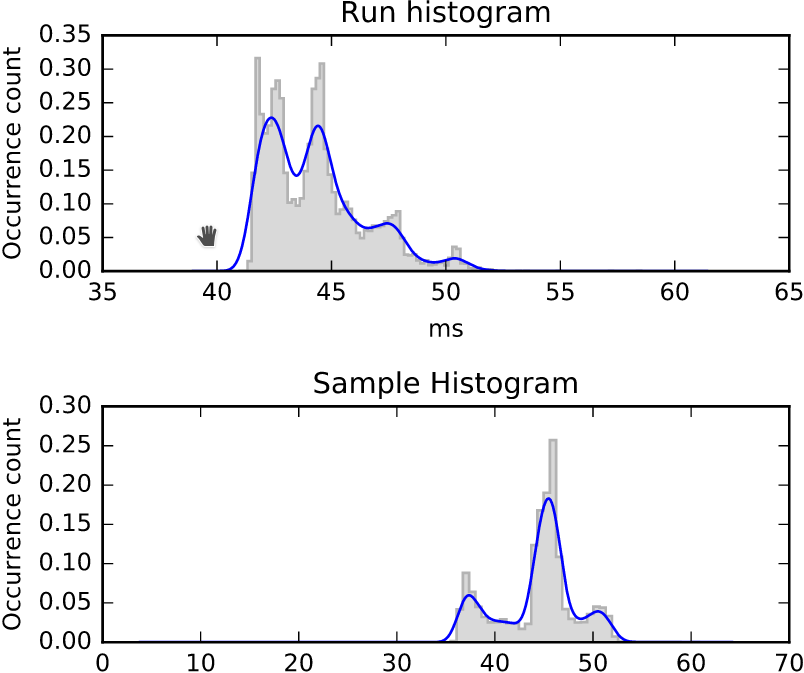
\includegraphics[width=5cm]{variance_bad.png} }}%
		\qquad
		\pause
		\subfloat[Good FPS distribution]{{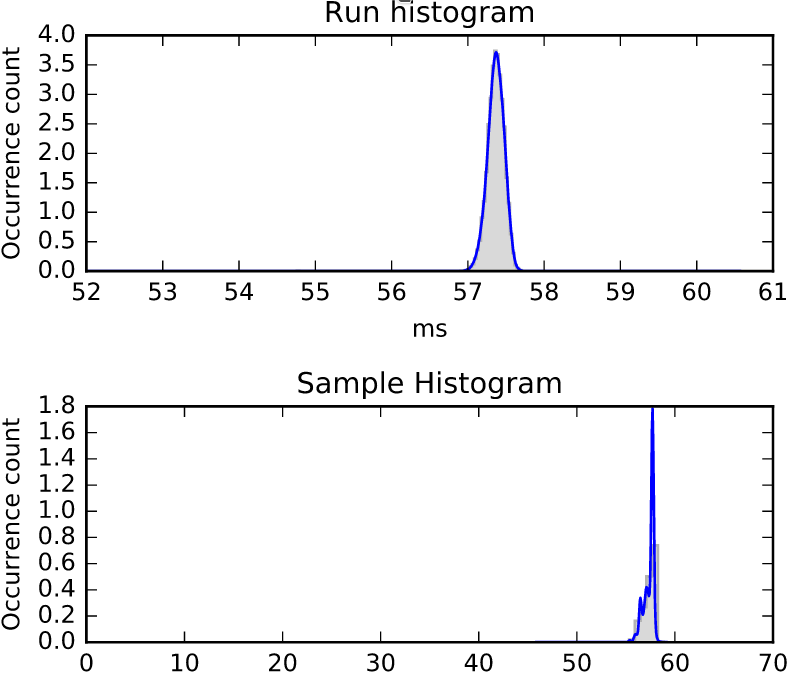
\includegraphics[width=5cm]{variance_good.png} }}%
		\caption{Examples of variance}%
	\end{figure}
\end{frame}

\begin{frame}
	\frametitle{EzBench: Handling variance}
	
	\begin{block}{Student-T test}
		Check if two data sets belong to the same normal distribution.
		\begin{figure}%
			\centering
			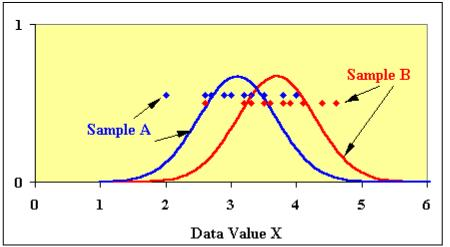
\includegraphics{tTestImage.jpg}
		\end{figure}
		
		\tiny Source: http://serc.carleton.edu/introgeo/teachingwdata/Ttest.html
	\end{block}
\end{frame}

\begin{frame}
	\frametitle{EzBench: Image comparaison}

	\begin{block}{Overview}
		\begin{itemize}
			\item Contributed by Pekka Jylhä-Ollila (Intel);
			\item Comparaison done using RMSE and requires 3 steps.
		\end{itemize}
	\end{block}
	
	\pause
	
	\begin{block}{Step 1: Comparing the output of 2 versions}
		\begin{figure}%
			\centering
			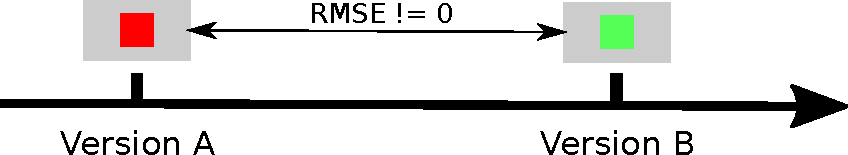
\includegraphics[width=\textwidth]{img_diff_step_1.pdf}
		\end{figure}
	\end{block}
\end{frame}

\begin{frame}
	\frametitle{EzBench: Image comparaison}

	\begin{block}{Step 2: Acquire more data and generate averages}
		\begin{figure}%
			\centering
			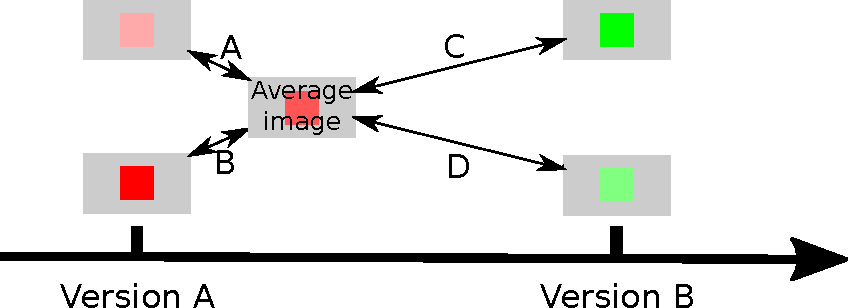
\includegraphics[width=\textwidth]{img_diff_step_2.pdf}
		\end{figure}
	\end{block}
	
	\pause
	
	\begin{block}{Step 3: Use the student-t test on the RMSEs}
		\begin{figure}%
			\centering
			
\includegraphics[width=\textwidth]{img_diff_step_3.pdf}
		\end{figure}
	\end{block}
\end{frame}

\begin{frame}
	\frametitle{EzBench: Demo time}

	\begin{block}{Demo 1: running loads with the simple runner}
		\begin{itemize}
			\item Listing tests;
			\item Running gtkperf in different environments;
			\item Showing the generated report;
			\item Start compiling a new version of mesa.
		\end{itemize}
	\end{block}
	
	\pause
	
	\begin{block}{Demo 2: Actual reports }
		\begin{itemize}
			\item Auto-bisected rendering change (5k commits, 7 months);
			\item Running gtkperf in different environments;
			\item Showing the generated report;
			\item Start compiling a new version of mesa.
		\end{itemize}
	\end{block}
\end{frame}

\begin{frame}
	\frametitle{EzBench: Needed features for CI}

	\begin{block}{Randomized testing}
		\begin{itemize}
			\item Not all tests can be run every day;
			\item Tests should be added randomly (as time permits);
		\end{itemize}
	\end{block}
	
	\pause
	
	\begin{block}{Support changing multiple components at the same time}
		\begin{itemize}
			\item EzBench needs to find the component that made the change;
			\item It thus needs to group data per environment;
			\item It needs to merge data from similar environments;
			\item It needs to be able to re-deploy environments;
			\item It needs to be able to recompile important components.
		\end{itemize}
	\end{block}
\end{frame}

\section{Conclusion}
\subsection*{Conclusion}
\begin{frame}
	\frametitle{Conclusion}
	
	\begin{block}{Ezbench's Goals}
		\begin{itemize}
			\item Automatically annotate a git tree with:
			\begin{itemize}
				\item Unit test results;
				\item Power and performance results;
				\item Rendering changes.
			\end{itemize}
			\item Require as little human intervention as possible;
			\item Provide reproducible results (environment).
		\end{itemize}
	\end{block}
	
	\pause
	
	\begin{block}{EzBench tries to take care of the pitfalls of benchmarking}
		\begin{itemize}
			\item Environment dumping and diffing;
			\item Reproduces results and tries to handle variance;
			\item Is reactive to changes, and self-improving;
			\item Handles most of the testing automatically.
		\end{itemize}
	\end{block}
\end{frame}

\begin{frame}[plain,c]
	\begin{center}
		\Huge Questions?
	\end{center}
\end{frame}

\section*{Backup slides}
\begin{frame}
	\frametitle{EzBench - Features}

	\begin{block}{Current features}
		\begin{itemize}
			\item Modular architecture (profiles, tests and user hooks);\pause
			\item Automates the acquisition of benchmark data;\pause
			\item Knows how long it is going to take;\pause
			\item Generates a report that is usable by developers;\pause
			\item Bisects performance changes automatically;\pause
			\item Provides python bindings to acquire data and parse reports;\pause
			\item Be crash-resistant by storing the expected goal and comparing it to the current state;\pause
			\item Collect the environment information and diff it;\pause
			\item Detect the variance and peformance changes;\pause
			\item Automatically schedule more work to improve the report.
		\end{itemize}
	\end{block}
\end{frame}

\begin{frame}
	\frametitle{EzBench - Features}

	\begin{block}{TODO}
		\begin{itemize}
			\item Watchdog support;\pause
			\item Handle kernel boot failures (need the watchdog);\pause
			\item Add support for PTS as a backend;\pause
			\item Better integrate the build process;\pause
			\item React to HW events such as throttling;\pause
			\item Reset the environment to a previous state;\pause
			\item Integrate with patchwork to test patch series;\pause
			\item Support sending emails to the authors of changes.
		\end{itemize}
	\end{block}
\end{frame}

\end{document}
